\documentclass[UTF8,a4paper,10pt]{ctexart}

\usepackage[left=1.0cm,right=1.0cm,top=0.74cm,bottom=0.84cm]{geometry}
\usepackage{fontspec}
\usepackage{xcolor}
\usepackage{graphicx}
\usepackage{tabularx}
\usepackage{array}
\usepackage{enumitem}
\usepackage{hyperref}

\IfFontExistsTF{Times New Roman}{\setmainfont{Times New Roman}}{}
\IfFontExistsTF{SimSun}{\setCJKmainfont{SimSun}}{}
\IfFontExistsTF{Microsoft YaHei}{\setCJKsansfont{Microsoft YaHei}}{}

\definecolor{resumeblue}{HTML}{0A5C7D}
\definecolor{resumeaccent}{HTML}{B7791F}
\definecolor{softline}{HTML}{D9E8EE}
\definecolor{textgray}{HTML}{4B5563}

\hypersetup{colorlinks=true, urlcolor=resumeblue}
\pagestyle{empty}
\setlength{\parindent}{0pt}
\setlength{\parskip}{0pt}
\setlength{\tabcolsep}{3.2pt}
\renewcommand{\arraystretch}{1.06}
\setlist[itemize]{leftmargin=1.3em, itemsep=0.07em, topsep=0.08em, parsep=0pt}
\setlist[enumerate]{leftmargin=1.5em, itemsep=0.06em, topsep=0.06em, parsep=0pt}

\newcolumntype{L}[1]{>{\raggedright\arraybackslash}p{#1}}
\newcolumntype{Y}{>{\raggedright\arraybackslash}X}

\newcommand{\sectiontitle}[1]{%
  \vspace{0.48em}
  {\sffamily\bfseries\Large\color{resumeblue}#1}\par
  \vspace{-0.28em}{\color{resumeblue}\rule{2.35cm}{1.05pt}}{\color{softline}\rule{\dimexpr\linewidth-2.35cm\relax}{1.05pt}}\vspace{0.13em}
}
\newcommand{\field}[2]{\textbf{#1：} & #2}
\newcommand{\entryhead}[3]{\textbf{#1} \hfill #2 \hfill \textbf{#3}}
\newcommand{\tightgap}{\vspace{-0.15em}}
\newcommand{\metriccell}[2]{{\sffamily\bfseries\color{resumeaccent}#1}\par{\fontsize{7.35pt}{9.2pt}\selectfont\color{textgray}#2}}

\begin{document}
\fontsize{9.05pt}{11.8pt}\selectfont

\begin{minipage}[t]{0.76\linewidth}
  {\sffamily\bfseries\fontsize{22pt}{25pt}\selectfont 王子成}
  \hspace{0.75em}
  {\sffamily\bfseries\fontsize{15.5pt}{19pt}\selectfont 长沙理工大学 电气与信息工程学院}\par
  \vspace{0.18em}
  {\color{resumeblue}\rule{\linewidth}{1.15pt}}\par
  \vspace{0.25em}
  {\sffamily\color{textgray}专业方向：新能源设备建模与电力系统稳定性分析 \quad AI+电力系统}\par
  \vspace{0.45em}
  \begin{tabularx}{\linewidth}{L{1.75cm}Y L{2.05cm}Y}
    \field{性别}{男} & \field{出生年月}{2005 年 10 月 20 日}\\
    \field{民族}{汉族} & \field{政治面貌}{入党积极分子}\\
    \field{籍贯}{安徽省亳州市蒙城县} & \field{居住地}{广东省深圳市}\\
    \field{电话}{19074917487} & \field{电子邮箱}{qqiuqiuhua@gmail.com / 202310080241@csust.com}\\
    \field{导师}{施星宇副教授、曹一家教授} & \field{班级职务}{文体委员}\\
  \end{tabularx}
\end{minipage}
\hfill
\begin{minipage}[t]{0.19\linewidth}
  \vspace{0.1em}
  \centering
  \setlength{\fboxsep}{2pt}
  \fcolorbox{softline}{white}{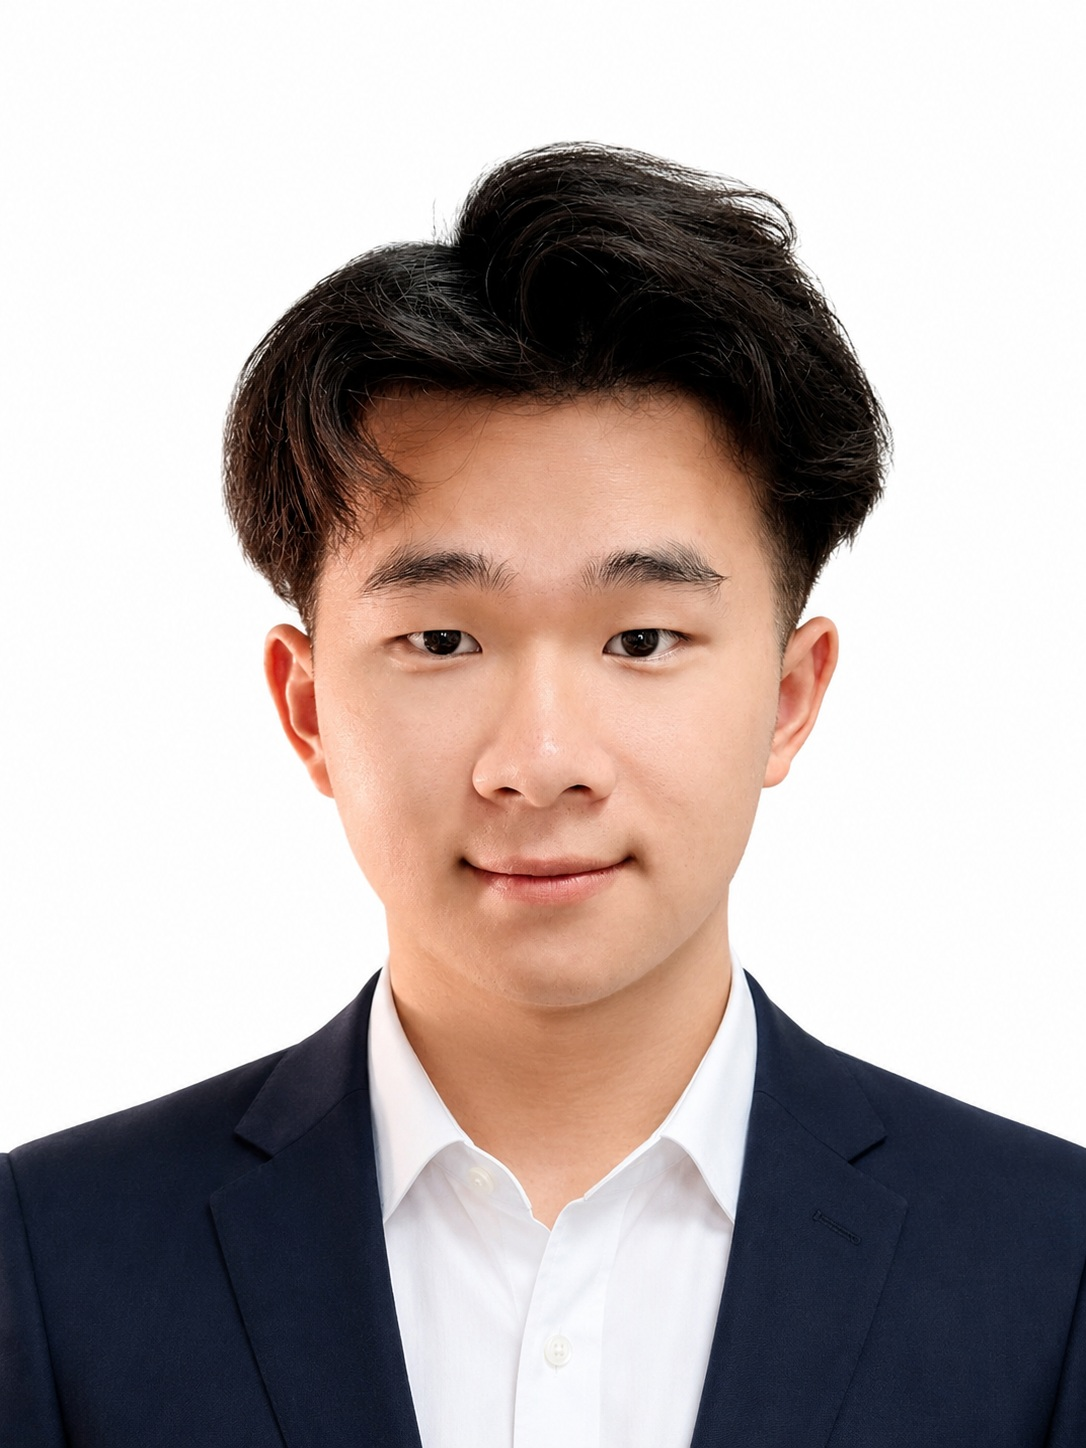
\includegraphics[width=3.0cm,height=3.85cm,keepaspectratio]{photo.jpg}}
\end{minipage}

\vspace{0.36em}
\begin{tabularx}{\linewidth}{>{\centering\arraybackslash}X>{\centering\arraybackslash}X>{\centering\arraybackslash}X>{\centering\arraybackslash}X}
\metriccell{综合测评前 2\%}{综合评价排名} &
\metriccell{第一作者论文 2 篇}{SCI 三区 + IEEE 会议} &
\metriccell{国家一等奖}{电工数学建模队长} &
\metriccell{软著 7 项}{授权 2 项 / 受理 5 项}
\end{tabularx}

\sectiontitle{综合能力}
\begin{tabularx}{\linewidth}{L{2.25cm}Y}
\textbf{专业方向} & 面向新能源并网稳定性问题，聚焦 PMSG 频域建模、阻抗/导纳预测、等效电路降阶与电力系统稳定性分析。\\
\textbf{成果产出} & 已形成第一作者 SCI 三区期刊论文 1 篇、IEEE 会议论文 1 篇；发明专利进入实质审查，软件著作权授权 2 项、受理 5 项。\\
\textbf{交叉基础} & 具备应用统计学大一数理训练与电气工程专业背景，兼具数学分析、高等代数、机器学习和电力系统仿真基础。\\
\textbf{综合表现} & 获电工杯全国大学生电工数学建模竞赛国家一等奖（队长）、金种子杯大学生创业大赛优胜奖（主要成员）、正大杯全国大学生市场调查与分析大赛湖南省一等奖（队员）。\\
\end{tabularx}

\sectiontitle{教育背景}
\begin{tabularx}{\linewidth}{L{3.0cm} L{5.1cm} L{3.8cm} Y}
\textbf{时间} & \textbf{学校/学院} & \textbf{专业} & \textbf{成绩与说明}\\
2024.09-2027.06 & 长沙理工大学电气与信息工程学院 & 电气工程及其自动化 & 本科在读（预计 2027.06 毕业）；截至大三上学期，平均学分成绩 87.02，GPA 3.46/4.0，学分绩点排名 103/424\\
2023.10-2024.06 & 长沙理工大学数学与统计学院 & 应用统计学 & 大一修读数学分析、高等代数、解析几何、微观经济学；后转入电气工程及其自动化专业\\
\end{tabularx}

\sectiontitle{学术成果}
\begin{tabularx}{\linewidth}{L{2.25cm}Y}
\textbf{发表论文} &
\begin{enumerate}
  \item 2026.05 | Wang Zicheng, et al. \textbf{Impedance Prediction of PMSG in Circuit Form Under Variable Operating Points}. ACPEE 2026, IEEE 会议论文，第一作者。
  \item 2026.05 | Wang Zicheng, et al. \textbf{Admittance Prediction for PMSG via Dimensionality-Reduced Equivalent Circuits and Support Vector Machines}. \textit{Technologies}, 2026, 14(6):323，中科院三区，第一作者。
\end{enumerate}\\[-0.55em]
\textbf{专利成果} & 2025.08 | 一种新能源系统频域建模与等效电路降阶分析方法，发明专利，实质审查。\\
\textbf{软件著作权} & 已授权 2 项：2025.08 基于阻抗参与因子的交直流混联输电系统振荡仿真与分析系统 V1.0；2025.10 常规矩阵变换器的故障诊断系统 V1.0。已受理 5 项：低碳电能与调频联合市场出清系统 V1.0；绿电直连型电氢氨园区优化运行系统 V1.0；新能源设备导纳智能预测与分析软件 V1.0；嵌入式社区养老服务站资源优化系统 V1.0；充电桩建设物资分类配送路径优化系统 V1.0。\\
\textbf{大创项目} & 基于阻抗参与因子的交直流混联输电系统振荡机理解析与弱阻尼环节定位，已结题。\\
\end{tabularx}

\sectiontitle{科研经历}
\entryhead{新能源设备阻抗/导纳建模与智能预测研究}{2025.01-至今}{第一作者论文方向}
\begin{itemize}
  \item 围绕 PMSG 变工况频域建模与稳定性分析，参与构建运行点采样、频域响应生成、等效电路参数降阶和机器学习预测流程，支撑第一作者 SCI/IEEE 论文产出。
  \item 结合降维等效电路与支持向量机方法，将高维频域特性映射为可解释电路参数，服务新能源并网稳定性快速建模与分析。
  \item 独立拆解学习构网/跟网解析模型与 Simulink 电磁暂态仿真模型，使用 MATLAB 搭建风机及逆变器稳态运行点模型，持续探索 Agent 与 PSCAD 交互建模。
\end{itemize}

\newpage
\sectiontitle{竞赛荣誉}
\begin{tabularx}{\linewidth}{L{2.25cm}L{10.95cm}Y}
\textbf{学科竞赛} & 2025.07.25 | 中国电机工程学会杯全国大学生电工数学建模竞赛 & 国家一等奖（队长）\\
 & 2025.05.03 | 美国大学生数学建模竞赛（MCM） & Successful Participant（世界级，队长）\\
 & 2026.06.29 | 全国大学生统计建模大赛 & 湖南省二等奖（队长）\\
 & 2025.08.01 | 全国大学生统计建模大赛 & 湖南省三等奖（队员）\\
 & 2026.05.01 | 全国大学生能源经济学术创意大赛 & 湖南省二等奖（队长）\\
 & 2025.12.01 | 全国大学生数学建模竞赛 & 湖南省三等奖（队长）\\
 & 2025.04.30 | 正大杯全国大学生市场调查与分析大赛 & 湖南省一等奖（队员）\\
 & 2025.12.05 | 中国国际大学生创新大赛（原互联网+） & 湖南省三等奖（队长）\\
 & 2026.06.03 | 金种子杯大学生创业大赛 & 优胜奖（主要成员）\\
 & 2024.12.15 | 湖南省普通本科高校一校一书一经典、精读、经世阅读推广活动 & 优秀读书报告二等奖（个人）\\[0.12em]
\textbf{奖学金} & 长沙理工大学学习科技竞赛奖单项奖学金；长沙理工大学优秀学生二等奖学金；长沙理工大学文艺活动优秀奖单项奖学金 & \\
\textbf{荣誉称号} & 长沙理工大学三好学生；长沙理工大学五四评优优秀团员；长沙理工大学五四评优社会实践先进个人 & \\
\end{tabularx}

\sectiontitle{技能水平}
\begin{tabularx}{\linewidth}{L{2.25cm}Y}
\textbf{英语水平} & CET-6 462 分，具备英文论文写作和国际会议英文口头汇报经历。\\
\textbf{专业能力} & 掌握新能源设备阻抗/导纳建模、电力系统稳定性分析、构网/跟网控制模型学习与拆解；能够使用 MATLAB 搭建风机及逆变器稳态运行点模型，并开展 Simulink/PSCAD 电磁暂态仿真学习与初步建模。\\
\textbf{编程建模} & 具备 MATLAB、Python/机器学习、深度学习与电力系统交叉建模经验，正在探索 Agent 与 PSCAD 交互自动生成仿真模型。\\
\textbf{软件工具} & 熟练使用 VS Code、MATLAB/Simulink、Office、Visio、EndNote、AxMath、TeXstudio、Codex；能够使用 SPSS、PSCAD 等专业分析与仿真软件。\\
\textbf{写作能力} & 具有 SCI 期刊论文、IEEE 会议论文、专利、软著材料、大创开题/结题报告等科研材料写作经验。\\
\textbf{综合素质} & C1 驾驶证；普通话二级乙等；兴趣特长包括视频剪辑、户外徒步与骑行。\\
\end{tabularx}

\sectiontitle{创新创业与实践}
\entryhead{长沙智碳联算科技有限责任公司}{2025.12.22-至今}{股东（持股 50\%）/软件开发}
\begin{itemize}
  \item 参与面向电力市场辅助服务、调频交易与市场出清分析场景的软件产品设计，负责合作关系协调、需求沟通与软件开发。
  \item 将业务侧调频服务需求转化为算法模块、软件功能和交付方案，积累电力市场、数据处理与工程软件开发经验。
\end{itemize}
\tightgap

\entryhead{沐风学习团队教育帮扶与学习互助实践}{2024.09.02-至今}{核心成员}
\begin{itemize}
  \item 作为长沙理工大学电网防灾减灾全国重点实验室沐风学习团队核心成员，参与面向本科生的学习互助、经验分享与教育帮扶工作。
  \item 团队长期组织课程答疑、科研入门分享和朋辈帮扶，相关事迹获长沙理工大学官微推送，并被多家媒体报道。
  \item 参与学习资源沉淀、活动组织与宣传协同，将个人科研训练、竞赛经验转化为面向低年级同学的可复用学习支持。
\end{itemize}
\tightgap

\entryhead{实践与志愿服务}{2025.11.30-至今}{社会实践}
\begin{itemize}
  \item 株洲大唐华银火力发电厂实习，了解火力发电生产流程、电气设备运行与安全管理要求，形成对传统电源侧运行逻辑和新能源并网问题的对照认识。
  \item 志愿服务时长超过 80 小时，参与校内外志愿服务与公益实践。
\end{itemize}

\sectiontitle{学生工作}
\begin{tabularx}{\linewidth}{L{3.0cm}L{4.95cm}L{2.15cm}Y}
2024.09-至今 & 电气工程及其自动化班级 & 文体委员 & 协助组织班级文体活动、赛事参与和集体建设工作，强化班级凝聚力与活动执行效率。\\
\end{tabularx}

\end{document}
